% TODO go back and rewrite the abstract
% TODO write equations for distance metric
% TODO write equations for majority metric

\documentclass{report}
\usepackage[utf8]{inputenc}
\usepackage{cite}
\usepackage{amsfonts}
\usepackage{amsmath}
\usepackage{algorithm, algpseudocode}
\usepackage{hyperref}
\usepackage{amssymb}
\usepackage{graphicx}
\graphicspath{{../pdf/}{D:}}


\title{Restaurant Recommendations using Collaborative Filtering}
\date{December\\ 2018}
\author{Michael Siem \\ \href{mailto:siem@wisc.edu}{siem@wisc.edu}
	\and Nathan Weinshenker \\ \href{mailto:nweinshenker@wisc.edu}{nweinshenker@wisc.edu}
	\and Jack Long \\ \href{mailto:jlong25@wisc.edu}{jlong25@wisc.edu}}

\begin{document}

\maketitle

\section*{Abstract}
With the growth of ecommerce and internet, predictions of user preferences is a hot topic in towards Machine Learning community. Our goal is to use Yelp's open data set \href {https://www.yelp.com/dataset/challenge} {Yelp Dataset Challenge} to compare two different methods—KNN and SVD-- towards implementing collaborative filtering to similar user preferences.  Our projects goal is 

%\section*{Data  Extraction}
%Our data required a lot of preprocessing where we acquired a conglomeration of user, business, and review date. In each data set, we have: 

\section*{Background Information}

Recommendation systems are a vital tool for providing users with personalized suggestions for items such as movies, music, and restaurants.
Product reviews data is widely accessible on services such as Spotify, Amazon, and Yelp.
There are two approaches that can be used to make recommendations to users based on this data, memory based, and model based. This activity will be focused on the former and touch briefly on the latter \cite{5}.
\newline

	
\subsection*{K Nearest Neighbors}
	
K Nearest Neighbors (k-NN) is a memory based collaborative filter that relies upon comparing features of a user or item to other users or items to receive a recommendation. 
k-NN is also a \textbf{non-parametric} learning algorithm. What non-parametric means is that k-NN has little or no prior knowledge about the data distribution. k-NN  builds the model structure based on the training data and this allows the algorithm to be highly versatile and simple to implement with little to no information about the data \cite{3}. 

\subsubsection*{History of Nearest Neighbors}

In 1992, Paul Resnick and fellow researchers at the University of Minnesota first studied collaborative filtering systems under the GroupLens project\cite{2}.  Collaborative filtering began to arise as a solution for dealing with overload in online information spaces. The first collaborative filtering system was Tapestry
a manual collaborative filtering system: it allowed the user to query for
items in an information domain, such as corporate e-mail, based on
other users’ opinions or actions\cite{6}. With the growth of the Internet, collaborative filters systems have grown in scope and popularity by big name tech companies like Netflix, Amazon, and Yahoo as predictive features for user-to-user 

\subsubsection{Nearest Neighbor Classification Derivation}
To understand k-NN, some necessary background information is required on probability. Here are some basic definitions of probability definitions. \cite{4}
\begin{enumerate}
	\item P(A | B), the conditional probability, is the probability of A given B
\end{enumerate}
Now lets assume that for  k-\textbf{nearest neighbor classification }  X = training data; Y = class labels of X; x = unknown sample.
Our k-nearest classifier will follow as:
Let $d$ be a distance measure (using euclidean distance)for our dataset $D$ where
\begin{equation}
D = (x_{1}, y_{1}), (x_{2}, y_{2}), ... , (x_{n}, y_{n})
\end{equation}
all the distance from x and D should be sorted in increasing distance , i.e,
$d(x,x_{i}) <= d(x,x_{i+1})$ \newline
The first $k \epsilon N$ points (where N is ordered distances) follow this  enumeration 
\begin{equation}
N_{k}(x) = (x_{1}, y_{1}), (x_{2}, y_{2}), ... , (x_{k}, y_{k}) 
\end{equation} 
\textsubscript{this is called a k-neighborhood of x (in D)}. \newline\newline
We will now define our classifier as 
\begin{equation}
\hat{p}(Y = y | x) = \frac{1}{k} \sum_{x',y' \epsilon N_{k}(x) }  I(y = y')
\end{equation}
and then we will predict the class of a user using the maximal predicted probability.
\begin{equation}
\hat{Y}(x) = argmin_{y \epsilon Y} \hat{p}(Y = y |x)
\end{equation}
\textsubscript{i.e., the majority class with repect to the classes of the neighbors}. \newline\newline

\subsubsection*{Classification Decision Rule}
Following determining the distance between test sample and training sample and the likelihood it's consider a neighbor, we can test it's classification.
With 1-nearest neighbor rule, the predicted class of test sample x is set equal to the true class y of its nearest neighbor, where mi is a nearest neighbor to x if the distance.
\begin{equation}
d(m_{i},x) = min_{j}(d(m_{j},x))
\end{equation}
Once all the test samples have been classified, the classification accuracy is based on the ratio of the number of correctly classified samples to the total number of samples classified, given in the form.
\begin{equation}
Accurary = \sum \frac{correctly classified}{total N}
\end{equation}
		


\subsubsection*{The Distance Function}

Several methods can be used to evaluate the distances between the neighbors and the point of interest.
We will first look at the use of the Euclidean distance or the straight-line distance between the points.

\begin{equation}
d(x_{i},x_{j}) = \sqrt{(x_{i1} - x_{j1})^2 + (x_{i2} - x_{j2})^2 + ... + (x_{ip} - x_{jp})^2}
\end{equation}

\subsubsection{K Nearest Neighbor Pseudocode }
\begin{algorithm}
  \caption{K Nearest Neighbour}
  \begin{algorithmic}
  	\State Classify (X,Y,x) // X:training data, Y: class labels of X, x:unknown sample
	\For{ t = 1 to T}
	\State Compute the distance between $d(X, x)$
	\State Sort all the distances in ascending order
	\EndFor
	\State Find the set Z containing indices for the k smallest distances $d(X_{i},x)$
	\State return the set of k closest points 
  \end{algorithmic}
\end{algorithm}


%\subsubsection*{Estimating the rating}
%At it's core, k-NN is a simple classification method where little or no prior knowledge about the distribution of the data is needed. K-nearest neighbor classification was first developed to perform discriminant analysis when estimates are unknown or difficult to determine. \textbf{include citation}
%	
%		
%Following determining the distance between test sample and training sample. 
%With 1 nearest neighbor rule, the predicted class of test sample is set equal to the true class of its nearest neighbor, where is a nearest neighbor to x if the distance 
%		
%$d(m_{i},x) = min_{j}(d(m_{j},x))$

		
%\subsubsection**{SVD Decomposition}
%		
%SVD is a matrix factorization technique that is usually used to reduce the number of features of a data set by reducing space dimensions from N to K where K < N. \\
%		
%Example matrix:
%			\[
%     			M=
%  				\begin{bmatrix}
%    					1 & 3 & ? & 3 & 1 \\
%    					3 & 2 & 5 & 8 & 7 \\
%    					3 & ? & 5 & ? & ? \\
%    					9 & ? & 3 & 2 & 1
%  				\end{bmatrix}
%			\]
%			\textit{ where M is sparse (i.e., “with missing entries”, not “containing a lot of zeros”)}
%			
%			
%			\begin{enumerate}
%				\item U is an n $x$ n orthogonal matrix
%				\item V is an d $x$ d orthogonal matrix
%				\item S is an n $x$ d diagonal matrix with nonnegative entries, and with the diagonal entries
%sorted from high to low 
%			\end{enumerate}
%			
%			A matrix with 




\section*{Warm-up}
Here are a couple activites to warm up on k-NN 
\begin{enumerate}
	\item The below data are 2D points with their classification. If we were to add the point (1,1) using 3-NN (K = 3) what would be the classification of this point?
	\begin{figure}[H]
		\centering
		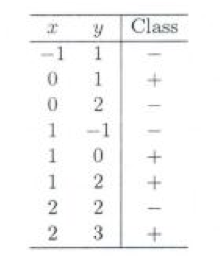
\includegraphics{../image/Picture1.png}
	\end{figure}
	\item Below is a diagram of points with classifications of either Red Triangle or Blue Square. A new point is introduced as the green circle. If the correct classification of the circle is Red Triangle, what k-values would misclassify this point? What does this tell us about having too large a k value
	\begin{figure}[H]
		\centering
		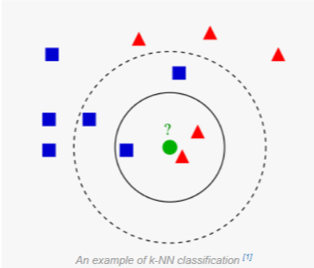
\includegraphics{../image/Picture2.png}
	\end{figure}
	\item How does raising the k value affect performance in data sets with a lot of noise? 
	\item Consider taking a 2D data set and then transforming it to fit into a 3D space. How would raising the dimension of K-NN effect the accuracy of the classifier?
	\item If the Minkowski distance is defined as: 
	\begin{equation}
	D (x, y) = ((\sum_{i}^{m}| x_{i} - y_{i}|^p)^\frac{1}{p})
	\end{equation}
     then when would you use Minkowski distance over Euclidean Distance?
	

\item Draw a Voronoi diagram
\end{enumerate}

\section*{Main Activity}

The main activity will be evaluating a KNN as a restaurant recommendation system using the Yelp dataset from \href{https://www.yelp.com/dataset}{https://www.yelp.com/dataset}.
The dataset originally contains 5,996,996 reviews for 188,593 businesses in 10 metropolitan areas.
We preprocessed the data set to narrow it down to 1 restaurant with 500 reviews for the activity, therefore we will be doing a user-user comparison.  
The activity will done using the Matlab script KNN.m.

\begin{enumerate}

\item Choosing K value

\item Evaluate different distance functions

\item Evaluate different classification metrics

\end{enumerate}

\section*{Future Work}
When classifying users some 

\begin {thebibliography}{999}
\bibliographystyle{plain}
	\bibitem{1}
	Leif E. Peterson
	Scholarpeida
	\href{http://www.scholarpedia.org/article/K-nearest_neighbor}{Scholarpedia}
	\bibitem{2}
	Joseph A. Konstan
    University of Minnesota
    Introduction to Recommender Systems
	\href{https://www-users.cs.umn.edu/~konstan/SIGMOD-2008-Tut.pdf}{UMN SIGMOD-2008}
	\bibitem{3}
	Benjamin Soltoff
    University of Chicago
    Statistical learning: non-parametric methods MACS-3100
	\href{https://cfss.uchicago.edu/persp010_nonparametric.html#objectives}{University Chicago MACS-3100}
	\bibitem{4}
	Lars Schmidt-Thieme
	 Institute for Computer Science University of Hildesheim
	 \href{https://www.ismll.uni-hildesheim.de/lehre/ml-07w/skript/ml-2up-03-nearest-neighbor.pdf} {K-NN Derivation}
	 \bibitem{5}
	Yifei Feng and Zhengli Sun
	Stanford University 
	Yelp User Rating
	 \href{http://cs229.stanford.edu/proj2014/Yifei%20Feng,%20Zhengli%20Sun,%20Yelp%20User%20Rating%20Prediction.pdf} {Link towards paper}
	 \bibitem{6}
	Collaborative Filtering Recommender Systems
	By Michael D. Ekstrand, John T. Riedl
	and Joseph A. Konstan
	 \href{http://files.grouplens.org/papers/FnT%20CF%20Recsys%20Survey.pdf} {Group Lens}
	 \bibitem{7}
	 R. Nowak
	 University of Wisconsin-Madison
	 ECE 830 Fall 2010 Statistical Signal Processing
	 \href{http://nowak.ece.wisc.edu/ece830/ece830_lecture24.pdf}{Signal Processing}
\end{thebibliography}
\end{document}


